\section{SPY: cómo opera STRATA, paso a paso}
\label{sec:mp-spy}

% Fuente única de cifras: notebooks/STRATA_marco_practico.ipynb (panel canónico de 10) y sus JSON en
% outputs/experiments/. Toda cifra trazada a su JSON en el caption de su tabla.

Empezamos por SPY, el ETF del S\&P~500. Es el caso que mejor deja ver el mecanismo: en un índice amplio la volatilidad alta coincide con las caídas del mismo día, de modo que el régimen lleva información de riesgo y el detector de régimen tiene contenido direccional. Es el \emph{leverage effect} (Black 1976 \cite{black1976}; Christie 1982 \cite{christie1982}), una coincidencia contemporánea: el régimen no predice la dirección de mañana, la acompaña hoy. Sobre este activo construimos toda la cadena: protocolo, calibración, los tres detectores, la intervención, las seis estrategias y los contrastes que separan lo que sobrevive de lo que no.

El agente solo (M5) acierta sobre SPY el $36{,}6\,\%$ de las direcciones, con un Sharpe de $-3{,}07$ y un capital final del $0{,}70$ del inicial. El \emph{sign test} contra $0{,}5$ (Conover 1999 \cite{conover1999}) rechaza la no-habilidad con $p < 0{,}001$ e intervalo de Wilson $[0{,}307,\ 0{,}429]$: el agente es un perdedor direccional, y ese es el problema que STRATA tiene que rescatar.

\subsection{Protocolo y calibración ex ante}
\label{sec:mp-spy-protocolo}

La causalidad es la del Capítulo~3, con \texttt{signal\_lag}${}=1$: la posición del día $t$ multiplica al retorno del día $t+1$, nunca al del propio día. Calibramos los tres detectores una sola vez sobre 2000-01-01 a 2024-09-30 y cerramos sus umbrales antes de mirar la evaluación, que arranca el 2024-10-01, después del corte de conocimiento del modelo de lenguaje. Dos ventanas conviven y nunca las mezclamos: el OOS completo ($n = 401$ días) sirve a las estrategias que no entrenan —agente, regla y las dos triviales—; la ventana desplegable ($n = 251$, tras un arranque de ciento cincuenta días de \emph{walk-forward} de origen rodante) es la de las que sí entrenan día a día, con embargo${}=1$ coherente con un horizonte de etiqueta de un día (Tashman 2000 \cite{tashman2000}; López de Prado 2018 \cite{lopezdeprado2018}). Comparar un modelo entrenado sobre $251$ días con una regla evaluada sobre $401$ sería mezclar peras y manzanas.

La Tabla~\ref{tab:mp-calib} recoge cada decisión con su criterio. El número de estados del HMM, $K = 3$, sale de una selección ex ante: la log-verosimilitud held-out por observación mejora de $-1{,}69$ con $K = 2$ a $-1{,}30$ con $K = 3$, y el BIC acompaña ($18\,775$ frente a $24\,131$). El estado más volátil tiene el retorno medio de calibración más bajo y el más tranquilo el más alto; esa gradación negativa vuelve el régimen un proxy de la dirección en un índice amplio (Rabiner 1989 \cite{rabiner1989}), y los etiquetamos Calma, Estrés y Crisis. La volatilidad la modelamos con un GARCH(1,1) de innovaciones $t$ de Student, que responde al exceso de curtosis de los retornos diarios (Bollerslev 1986 \cite{bollerslev1986}); el cambio estructural lo seguimos con BOCPD \emph{online}, que en cada paso actualiza la probabilidad del último cambio sin usar información posterior (Adams y MacKay 2007 \cite{adams2007}). Los tres umbrales son cuantiles de la calibración: RAM $\tau = 0{,}50$, PSA $P_{95} = 0{,}023$ y GSO $P_{95} = 2{,}371$.

\begin{table}[htbp]
\centering
\caption{Decisiones de calibración de STRATA sobre SPY, con su criterio de fijación. Todas se cierran sobre 2000-01-01 a 2024-09-30, antes de la evaluación. Fuente: \texttt{k\_selection.json}, \texttt{cache/models/strata\_thresholds.json}.}
\label{tab:mp-calib}
\begin{tabular}{lll}
\toprule
Decisión & Valor & Criterio (cita) \\
\midrule
Estados del HMM & $K = 3$ & held-out $-1{,}30 > -1{,}69$; BIC $18\,775 < 24\,131$ \cite{rabiner1989} \\
Volatilidad & GARCH(1,1)-$t$ & colas pesadas de los retornos \cite{bollerslev1986} \\
Cambio estructural & BOCPD \emph{online} & causalidad de la alarma \cite{adams2007} \\
Umbral RAM & $\tau = 0{,}50$ & voto de mayoría del régimen \\
Umbral PSA & $P_{95} = 0{,}023$ & cuantil de calibración \\
Umbral GSO & $P_{95} = 2{,}371$ & cuantil de calibración \\
\bottomrule
\end{tabular}
\end{table}

El \emph{leverage} de un activo lo medimos con la correlación de Black, $\mathrm{lev} = \operatorname{corr}(r_t,\ \mathrm{RV}^{21}_{t+1} - \mathrm{RV}^{21}_t)$, negativa cuando una caída de hoy eleva la volatilidad de mañana. La Figura~\ref{fig:mp-regimenes-spy} pinta los tres regímenes sobre el precio. Una precisión gobierna toda la lectura que sigue: en calibración el retorno del mismo día baja con el régimen, pero la fracción de días al alza del día siguiente ronda $0{,}5$ incluso en Crisis. El régimen separa por volatilidad y coincide con las caídas el mismo día; no anticipa el signo de mañana, y por eso su valor está en disciplinar el riesgo, no en predecir.

\begin{figure}[htbp]
\centering
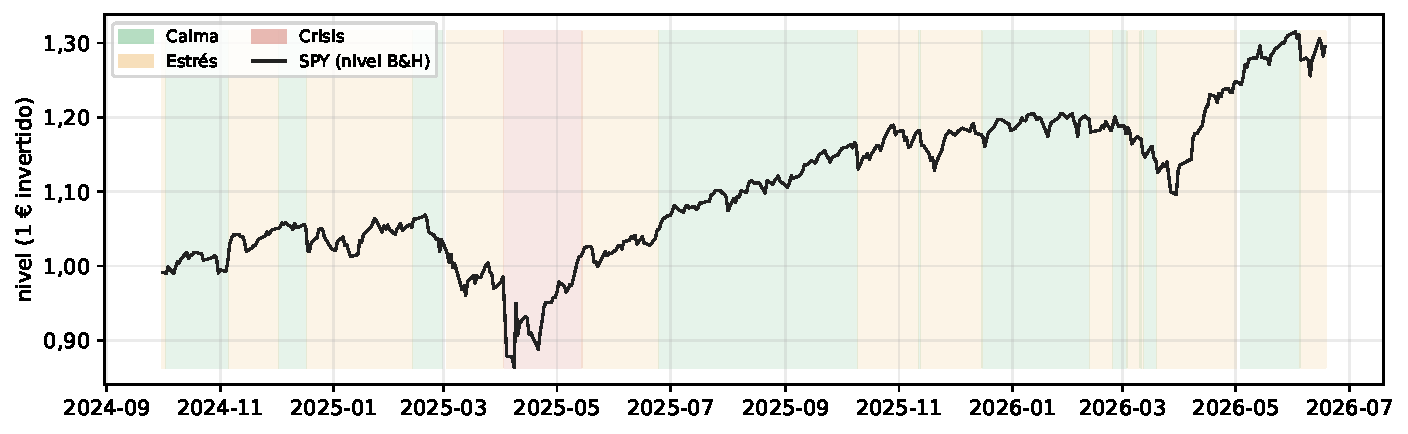
\includegraphics[width=0.9\textwidth]{figuras/cap4_regimenes_spy}
\caption{Regímenes del HMM ($K = 3$) sobre el precio de SPY en el periodo de evaluación. Calma (volatilidad baja, retorno medio positivo), Estrés (intermedio) y Crisis (volatilidad alta, retorno medio negativo) ordenan por la firma del \emph{leverage effect}. El sombreado marca el régimen vigente cada día; la coincidencia régimen$\leftrightarrow$caída es contemporánea, no predictiva. Fuente: \texttt{regime\_direction\_table.json}.}
\label{fig:mp-regimenes-spy}
\end{figure}

\subsection{Los tres detectores y la intervención}
\label{sec:mp-spy-detectores}

Los tres detectores miran ejes ortogonales. RAM lee el régimen y comprueba si la dirección de la apuesta concuerda con el estado vigente: su \emph{score} es la probabilidad que el HMM pone en que el agente apuesta contra el régimen, y dispara cuando $\mathrm{RAM}_t \ge \tau = 0{,}50$. PSA vigila con BOCPD si el agente cambia de criterio de forma estructural (Adams y MacKay 2007 \cite{adams2007}); GSO contrasta el tamaño de la posición con la volatilidad del GARCH (Bollerslev 1986 \cite{bollerslev1986}). Cuando RAM dispara, la intervención reorienta la posición al signo del régimen, fijado por un prior calibrado por activo —la media del retorno de cada estado—, nunca por una regla escrita a mano del tipo ``Crisis implica corto''.

Sobre SPY actúa una sola supervisión (Tabla~\ref{tab:mp-detectores}). RAM dispara el $30{,}2\,\%$ de los días: de las ciento veintiuna intervenciones, setenta y una aciertan y cincuenta fallan. PSA dispara dos días y GSO ninguno, porque el agente mantiene una posición casi constante sobre SPY (corto la mayor parte de los días) y sus \emph{scores} de cambio y de tamaño quedan por debajo de los umbrales. Son detectores inertes como reglas sobre este activo, y lo registramos. El rescate acumulado, $+0{,}312$, sale entero de los días en que RAM dispara; PSA y GSO aportan exactamente cero.

\begin{table}[htbp]
\centering
\caption{Actividad de los tres detectores sobre el OOS completo de SPY ($n = 401$ días). ``Acierto'' es la fracción de direcciones correctas en los días en que el detector dispara; el P\&L de rescate es el acumulado de la intervención en esos días. PSA y GSO apenas disparan: su columna de acierto no aplica. Fuente: \texttt{spy\_intervention\_anatomy.json}.}
\label{tab:mp-detectores}
\begin{tabular}{lrrrr}
\toprule
Detector & Tasa de disparo & Acierto M8 & Acierto M5 & P\&L de rescate \\
\midrule
\textbf{RAM} (régimen) & $\mathbf{30{,}2\,\%}$ & $\mathbf{0{,}587}$ & $0{,}413$ & $\mathbf{+0{,}312}$ \\
PSA (cambio estructural) & $0{,}5\,\%$ & --- & --- & $0{,}000$ \\
GSO (volatilidad) & $0{,}0\,\%$ & --- & --- & $0{,}000$ \\
\bottomrule
\end{tabular}
\end{table}

Que RAM acierte al intervenir no es casualidad, y la Figura~\ref{fig:mp-scores-detectores} lo deja ver. En los días en que RAM está alto, seguir el régimen bate a seguir al agente ($0{,}587$ frente a $0{,}413$); cuando RAM está bajo, la ventaja se diluye y la intervención no se activa. El detector funciona como una compuerta: deja pasar la decisión del agente salvo cuando choca con el régimen, y solo entonces la corrige. En SPY esa compuerta es todo el mecanismo, porque el canal de régimen es el único que se enciende.

\begin{figure}[htbp]
\centering
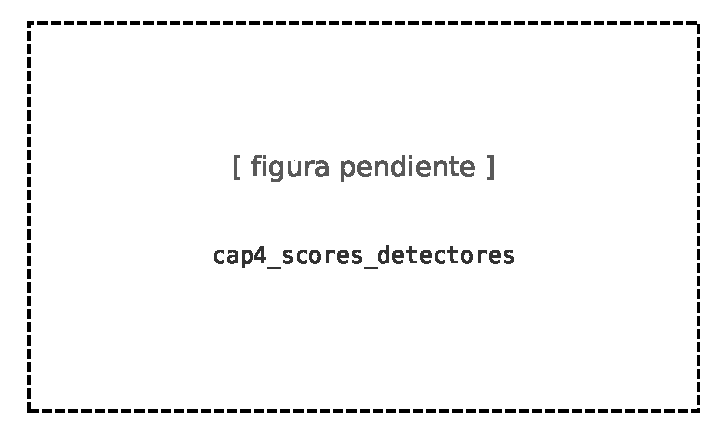
\includegraphics[width=0.9\textwidth]{figuras/cap4_scores_detectores}
\caption{Distribución de los \emph{scores} de RAM, PSA y GSO sobre el OOS de SPY, con su umbral de disparo marcado (RAM $\tau = 0{,}50$, PSA $P_{95} = 0{,}023$, GSO $P_{95} = 2{,}371$). El \emph{score} de RAM es bimodal y cruza el umbral con frecuencia; los de PSA y GSO se acumulan muy por debajo del suyo, de ahí que apenas disparen. Fuente: \texttt{spy\_intervention\_variants.json}.}
\label{fig:mp-scores-detectores}
\end{figure}

\subsection{Anatomía de la intervención y elección del modo}
\label{sec:mp-spy-variantes}

La intervención puede ejecutarse de tres maneras, y la elección no es cosmética: abstenerse los días dudosos (cerrar la posición), reducir el tamaño a la mitad, o reorientar la dirección al signo del régimen —el modo \emph{override}—. La Tabla~\ref{tab:mp-variantes} los compara sobre los días en mercado ($n = 232$). El \emph{override}, que adoptamos como canónico, acierta el $47{,}8\,\%$; abstenerse el $40{,}1\,\%$ y reducir el $39{,}7\,\%$, indistinguible del agente sin tocar. El Sharpe acompaña: $-0{,}46$ del \emph{override} frente a $-2{,}10$ de abstenerse y $-2{,}75$ de reducir. El valor está en corregir activamente la dirección cuando choca con el régimen, no en limitarse a evitar el riesgo.

\begin{table}[htbp]
\centering
\caption{Modos de intervención de M8 sobre SPY (días en mercado, $n = 232$). El modo canónico (\emph{override}) reorienta la posición al signo del régimen; las alternativas se abstienen o reducen el tamaño. En negrita, el modo adoptado. Fuente: \texttt{spy\_intervention\_variants.json}.}
\label{tab:mp-variantes}
\begin{tabular}{lrrr}
\toprule
Modo & Accuracy & Sharpe & Capital \\
\midrule
\textbf{Override} (canónico) & $\mathbf{0{,}478}$ & $\mathbf{-0{,}46}$ & $\mathbf{0{,}94\times}$ \\
Abstención & $0{,}401$ & $-2{,}10$ & $0{,}81\times$ \\
Reducir a la mitad & $0{,}397$ & $-2{,}75$ & $0{,}75\times$ \\
M5 (agente sin tocar) & $0{,}397$ & $-3{,}07$ & $0{,}70\times$ \\
\bottomrule
\end{tabular}
\end{table}

La anatomía de esas ciento veintiuna intervenciones está en la matriz de confusión de la Figura~\ref{fig:mp-confusion-spy}: en setenta y un casos el agente apostaba contra el régimen y la intervención lo corrige; en cincuenta tenía razón y la intervención mete ruido. El saldo neto es positivo porque la intervención no es indiscriminada: crece con la discrepancia entre la apuesta del agente y el signo del régimen, y son justo esos días de discrepancia grande los que aportan el grueso del rescate.

\begin{figure}[htbp]
\centering
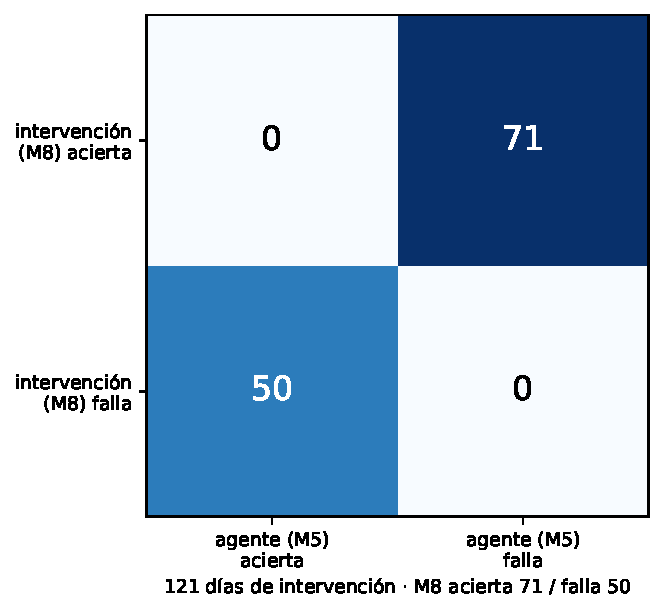
\includegraphics[width=0.7\textwidth]{figuras/cap4_confusion_spy}
\caption{Matriz de confusión de la intervención sobre SPY: dirección del agente (M5) frente a dirección tras intervenir (M8), sobre las $121$ intervenciones. La diagonal de rescate ($71$ aciertos de la intervención cuando el agente fallaba) supera a la de daño ($50$). Fuente: \texttt{spy\_intervention\_anatomy.json}.}
\label{fig:mp-confusion-spy}
\end{figure}

\subsection{Las seis estrategias: accuracy, riesgo y la trivial}
\label{sec:mp-spy-estrategias}

Comparamos seis estrategias. M5 es el agente sin supervisar; M8, la regla determinista de la intervención; M10, el meta-learner, un ensemble de diez XGBoost sobre las veintidós características del agente y de STRATA; AutoML deja que H2O busque por reentreno entre GBM, XGBoost y su apilamiento. Las dos referencias triviales —comprar y mantener (B\&H) y la clase mayoritaria del pasado (ZeroR)— marcan el listón que cualquier pretensión de habilidad debe superar. La Tabla~\ref{tab:mp-spy} las reúne sobre la ventana desplegable.

\begin{table}[htbp]
\centering
\caption{Las seis estrategias sobre SPY, ventana desplegable ($n = 251$, \texttt{signal\_lag}${}=1$). Accuracy direccional, Sharpe anualizado, máxima caída, ratio de Calmar (Young 1991 \cite{young1991}) y capital final por euro invertido. En negrita, la mejor en cada columna. Fuente: \texttt{automl\_runs/panel\_mm25\_inclGBM-XGB-SE\_AUC\_emb1\_N0-150\_step21\_kfold\_seed42.json}.}
\label{tab:mp-spy}
\begin{tabular}{lrrrrr}
\toprule
Estrategia & Accuracy & Sharpe & Máx.\ caída & Calmar & Capital \\
\midrule
\textbf{AutoML} (búsqueda H2O) & $\mathbf{0{,}574}$ & $\mathbf{+2{,}68}$ & $\mathbf{-5{,}5\,\%}$ & $\mathbf{6{,}93}$ & $\mathbf{1{,}38\times}$ \\
ZeroR (clase mayoritaria) & $0{,}566$ & $+2{,}21$ & $-9{,}8\,\%$ & $3{,}10$ & $1{,}30\times$ \\
B\&H (comprar y mantener) & $0{,}566$ & $+2{,}21$ & $-9{,}8\,\%$ & $3{,}10$ & $1{,}30\times$ \\
M10 (meta-learner XGBoost) & $0{,}494$ & $-0{,}60$ & $-16{,}1\,\%$ & $-0{,}50$ & $0{,}92\times$ \\
M8 (regla STRATA) & $0{,}442$ & $-0{,}46$ & $-15{,}2\,\%$ & $-0{,}39$ & $0{,}94\times$ \\
M5 (agente solo) & $0{,}366$ & $-3{,}07$ & $-30{,}2\,\%$ & $-1{,}00$ & $0{,}70\times$ \\
\bottomrule
\end{tabular}
\end{table}

Leída de abajo arriba, cada capa rescata al agente. M8 sube la accuracy de $0{,}366$ a $0{,}442$ y recorta la máxima caída del $30{,}2\,\%$ al $15{,}2\,\%$; M10 llega a $0{,}494$; AutoML alcanza $0{,}574$ y gana en todas las columnas, también a las dos triviales, con un Sharpe de $+2{,}68$ frente a $+2{,}21$ del pasivo y una máxima caída de solo el $5{,}5\,\%$. El McNemar pareado (McNemar 1947 \cite{mcnemar1947}) sobre los aciertos diarios mide la significancia del rescate: $p = 0{,}0002$ para AutoML frente a M5, $p = 0{,}0074$ para M10 y $p = 0{,}051$ para M8. Los tres rescatan al agente, y el rescate es significativo.

La victoria sobre la trivial pide un matiz. El mismo McNemar de AutoML frente a ZeroR da $p = 0{,}90$: no hay potencia para separarlos en doscientos cincuenta días. La ventaja de AutoML sobre el pasivo es real en punto pero nominal en significancia, y tiene explicación económica: SPY es mayormente beta de mercado, el periodo fue alcista, e ir largo capturó esa subida. La gráfica de equity de la Figura~\ref{fig:mp-equity-spy} hace visible la diferencia, y el Sharpe deflactado (López de Prado 2018 \cite{lopezdeprado2018}; Bailey y López de Prado 2014 \cite{bailey2014}) la pone en contexto: el DSR de AutoML es $0{,}92$, frente a $0{,}05$ de M10 y $0{,}00$ del agente. AutoML es el único modelo cuyo Sharpe sobrevive al ajuste por número de pruebas.

\begin{figure}[htbp]
\centering
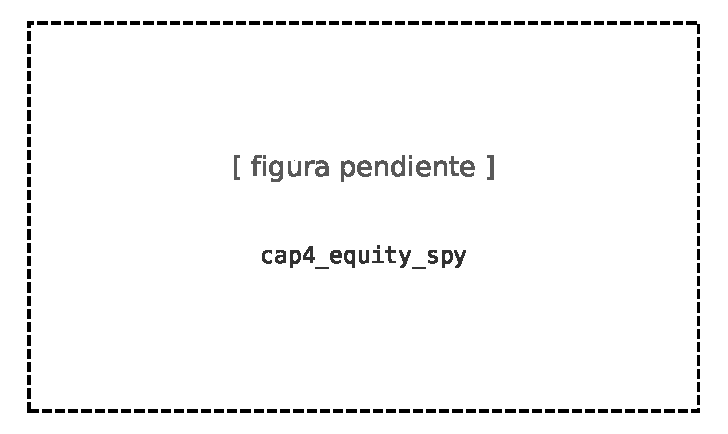
\includegraphics[width=0.9\textwidth]{figuras/cap4_equity_spy}
\caption{Curvas de capital de las seis estrategias sobre SPY (ventana desplegable, $n = 251$ días, un euro inicial). AutoML (línea destacada) supera a las dos referencias triviales en Sharpe ($+2{,}68$ frente a $+2{,}21$), en máxima caída ($-5{,}5\,\%$ frente a $-9{,}8\,\%$) y en capital final ($1{,}38\times$ frente a $1{,}30\times$); el agente solo (M5) termina en $0{,}70\times$. La ventaja sobre la trivial es nominal (McNemar AutoML vs ZeroR $p = 0{,}90$). Fuente: \texttt{automl\_net\_returns.json}.}
\label{fig:mp-equity-spy}
\end{figure}

Hay un resultado en riesgo que no alcanza significancia a este nivel: sobre un único activo, el intervalo de confianza del $\Delta$Sharpe de la regla frente al agente cruza el cero. La prueba dura del rescate en riesgo vive en la agregación del panel, y la damos en la Sección~\ref{sec:mp-panel}.

\subsection{Robustez del caso SPY: ablación y anti-tuning}
\label{sec:mp-spy-robustez}

¿Usa de verdad el aprendiz las señales de STRATA, o gana por otro lado? Al quitar PSA y GSO de las características, AutoML baja de $0{,}574$ a $0{,}550$ en accuracy (Tabla~\ref{tab:mp-ablacion}): aunque PSA y GSO casi no disparen como reglas, sus \emph{scores} continuos informan al modelo. Las características de Shapley (Lundberg y Lee 2017 \cite{lundberg2017}) lo confirman, y etiquetamos cada cuota con su modelo y su ventana porque no son el mismo objeto. Sobre el ensemble M10 ($n = 251$) la cuota de las features de STRATA es $0{,}71$; sobre el \emph{leader} de AutoML ($n = 401$) es $0{,}565$ por árbol y $0{,}564$ por permutación. Las dos superan la mitad y colocan los detectores por delante de las características del propio agente.

\begin{table}[htbp]
\centering
\caption{Ablación de detectores sobre SPY (ventana desplegable, $n = 251$). El conjunto canónico usa las veintidós características; ``sin PSA+GSO'' deja solo el canal de régimen entre los detectores. AutoML degrada al quitar PSA+GSO, prueba de que usa sus \emph{scores}. Fuente: \texttt{automl\_ablation\_detectors.json}, \texttt{detector\_ablation\_panel.json}.}
\label{tab:mp-ablacion}
\begin{tabular}{lrr}
\toprule
Conjunto de características & Accuracy AutoML & Accuracy M10 \\
\midrule
\textbf{ALL22} (canónico) & $\mathbf{0{,}574}$ & $0{,}494$ \\
sin PSA+GSO & $0{,}550$ & $0{,}514$ \\
\bottomrule
\end{tabular}
\end{table}

La objeción más natural es que los umbrales se eligieran para que el resultado saliera bien. El barrido lo descarta (Figura~\ref{fig:mp-sensibilidad}): la accuracy de M8 frente al umbral RAM es plana en una meseta, $0{,}466$ en $\tau = 0{,}3$ y $0{,}478$ a partir de $\tau = 0{,}5$, sin saltos, y la del meta-learner frente a su umbral de decisión también es plana en torno a $0{,}50$. El resultado no cuelga de un punto afortunado del espacio de hiperparámetros: descansa sobre una región estable, lo contrario de un ajuste fino al periodo de evaluación. Esta meseta es nuestra mejor defensa frente a la sospecha de sobreajuste.

\begin{figure}[htbp]
\centering
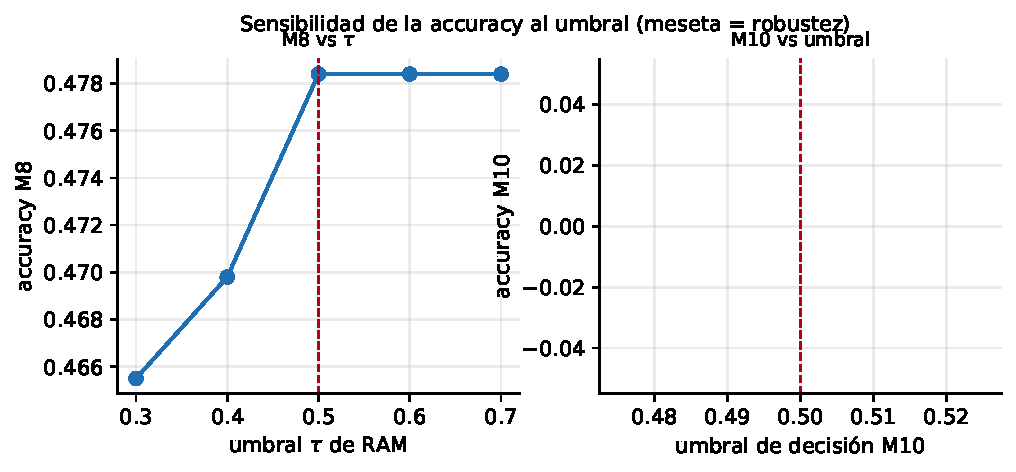
\includegraphics[width=0.9\textwidth]{figuras/cap4_sensibilidad_umbrales}
\caption{Sensibilidad de la accuracy al umbral de decisión sobre SPY: M8 frente a $\tau$ del detector RAM y M10 frente a su umbral de probabilidad. Las dos curvas son planas en una meseta alrededor del valor canónico (marcado), señal de robustez y no de ajuste a un punto. Fuente: \texttt{psa\_gso\_threshold\_sensitivity.json}.}
\label{fig:mp-sensibilidad}
\end{figure}

Sobre SPY el mecanismo es transparente y el agente, solo, pierde con holgura. La intervención por régimen lo corrige y la derivada aprendida supera a la trivial en este punto, apoyándose en las señales de STRATA y sobre una meseta robusta de umbrales. A nivel de un único activo, sin embargo, la corrección de riesgo no alcanza significancia y la victoria sobre la trivial es nominal. Para probar el rescate hace falta salir de SPY: el panel de diez activos es el siguiente paso.
